\documentclass[10pt, conference, compsocconf]{llncs}
% Add the compsocconf option for Computer Society conferences.
%
% If IEEEtran.cls has not been installed into the LaTeX system files,
% manually specify the path to it like:
% \documentclass[conference]{../sty/IEEEtran}
\newcommand{\highlight}[1]{\colorbox{yellow}{#1}}


% Some very useful LaTeX packages include:

% *** MISC UTILITY PACKAGES ***
%
\usepackage{ifpdf}


% *** CITATION PACKAGES ***
%
%\usepackage{cite}


% *** MATH PACKAGES ***
%
\usepackage[cmex10]{amsmath}
\usepackage{amssymb}

% *** SPECIALIZED LIST PACKAGES ***
%
\usepackage{algorithmic}

% *** ALIGNMENT PACKAGES ***
%
\usepackage{array}

% *** SUBFIGURE PACKAGES ***
%
\usepackage[tight,footnotesize]{subfigure}

% *** FLOAT PACKAGES ***
%
\usepackage{fixltx2e}
\usepackage{stfloats}

% *** GRAPHICS PACKAGES ***
%
\usepackage{graphicx}

% *** BIBLIOGRAPHY PACKAGES ***
%
\usepackage{natbib}

% *** LANGUAGE PACKAGES ***
%
\usepackage[utf8]{inputenc} 
\usepackage[T1]{fontenc}      
\usepackage[francais]{babel}

% *** LAYOUT PACKAGES ***
%
\usepackage[top=4cm, bottom=4cm, left=4cm, right=4cm]{geometry}


\begin{document}
%
% paper title
% can use linebreaks \\ within to get better formatting as desired
\title{Le numérique dans\\l'accomplissement des SDGs}





% author names and affiliations
% use a multiple column layout for up to two different
% affiliations
% 
\author{Djavan Sergent \\
Master en Sciences Informatiques \\
 \{djavan.sergent@etu.unige.ch\}}

\institute{Université de Genève}



% make the title area
\maketitle


\begin{abstract}
	<ABSTRACT>
\end{abstract}


\textbf{Mots clés}
MDG; SDG; Citizen Science ; Monitoring ; Biodiversity ; Water Quality ; United Nations ; Sustainable Development


\section{Introduction}
	En 2000, les Nations-Unies lancent le programme des Millenim Developpment Goals (MDGs) qui s'étend jusq'en 2015 \cite{united_nations_millennium_2009}. Il s'agit d'un ensemble d'objectifs internationaux parmi lesquels on peut notamment citer l'éradication de l'extrême pauvreté et de la faim, combattre la mortalité infantile ou encore apporter une éducation à toutes et tous. Les 191 états membres des Nations-Unies ainsi que 22 organisations internationnales se sont engagées à participer activement à la réalisation de ces objectifs \cite{wikipedia_millennium_2017}.
	\begin{figure}
		\begin{center}
			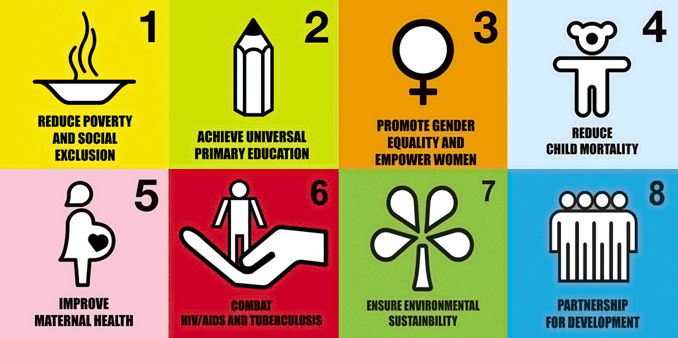
\includegraphics[width=200pt]{mdgs-full.png}
		\end{center}
		\caption{Représentation des MDGs (source : Wikipedia)}
	\end{figure}
	
	La situation en 2015 était que beaucoup d'efforts ont été investis, mais les progrès sont encore très inégaux. Les différents pays membres des Nations-Unies ainsi que des organisations civiles se sont donc intéressées à l'agenda post-2015, c'est à dire aux objectifs futurs. Les Sustainable Developpment Goals (SDGs) ont étés acceptés comme relève des MDGs \cite{wikipedia_sustainable_2017}. Ceux-ci comportent 17 buts, chacuns subdivisé en objectifs. Les SDGs totalisent 169 objectifs possédant chacuns leurs propres indicateurs.
	\begin{figure}
		\begin{center}
			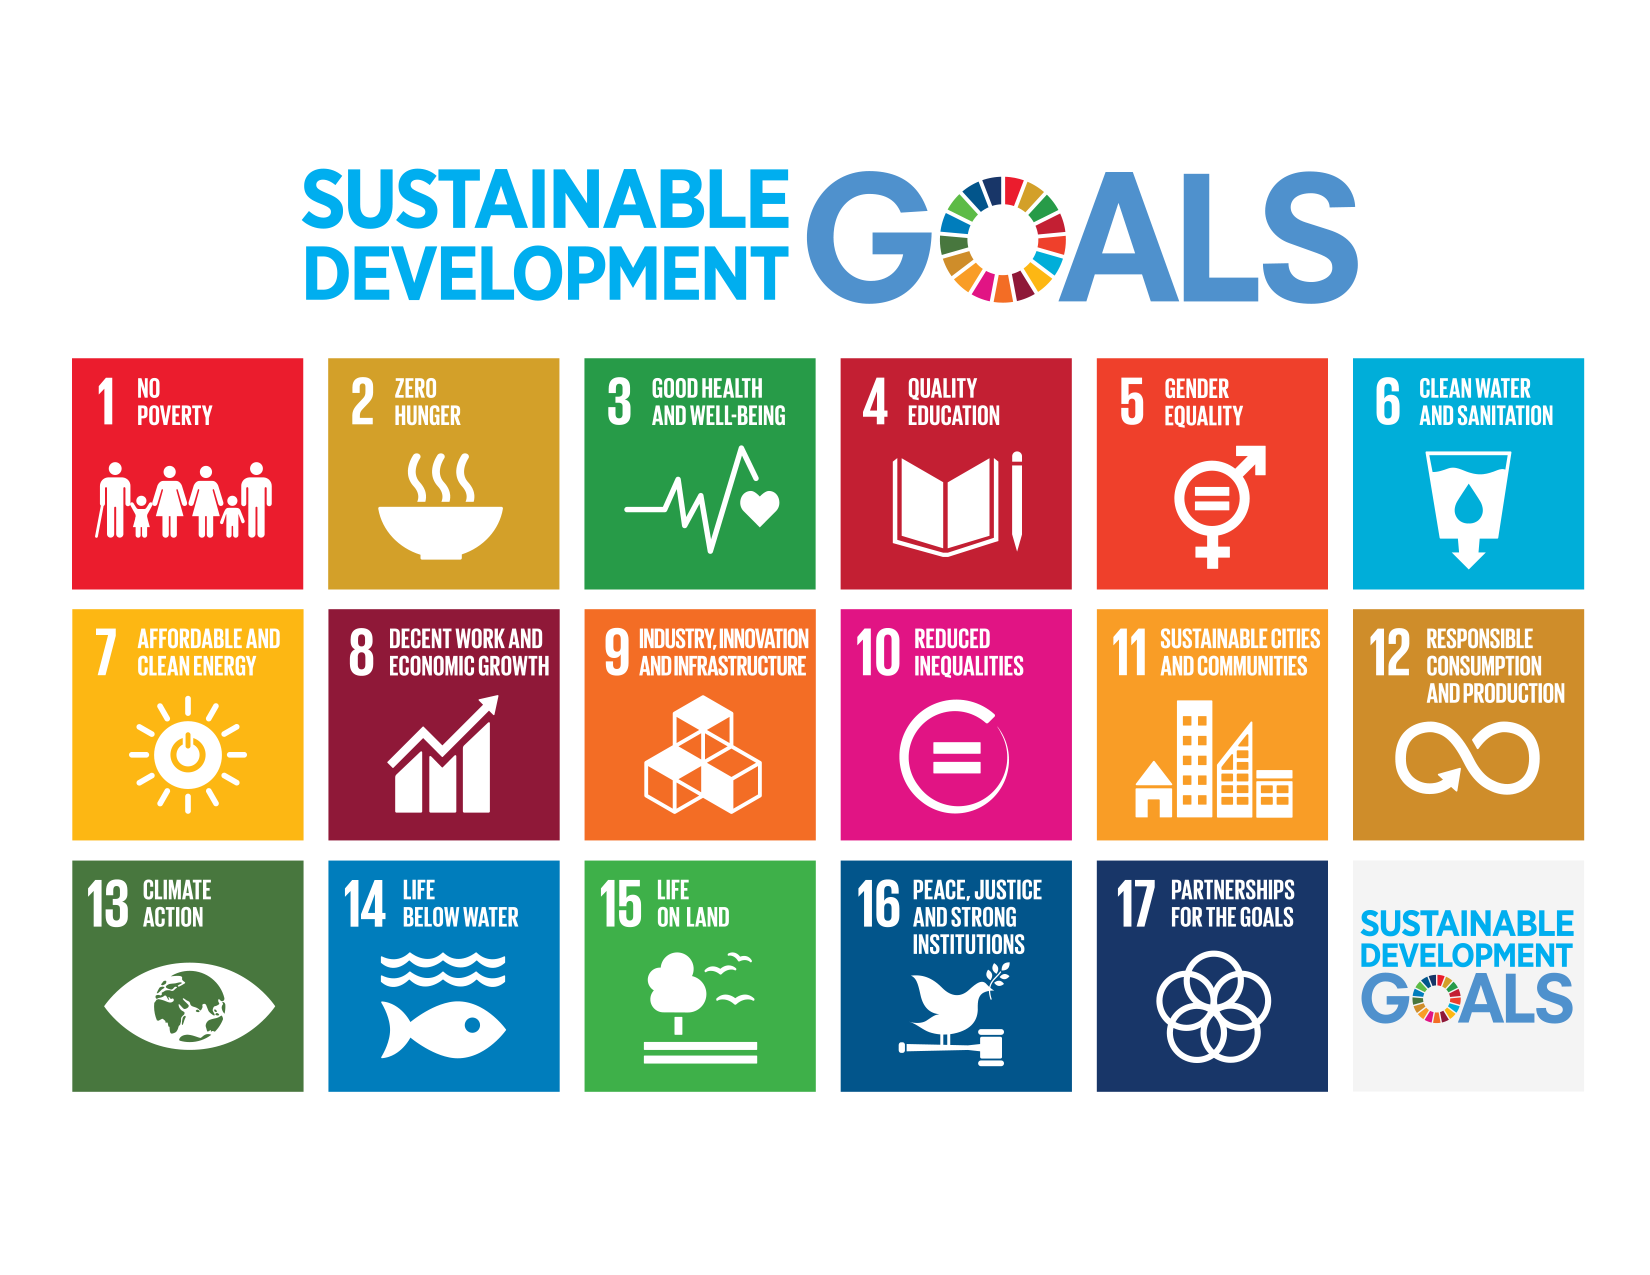
\includegraphics[width=200pt]{sdgs.jpg}
		\end{center}
		\caption{Représentation des SDGs (source : Wikipedia)}
	\end{figure}
	\\
	Nous analysons dans cet article le rôle du numérique dans la réalisation et le monitoring de certains de ces objectifs, particulièrement du point de vue de la participation citoyenne.

	\subsection{Sustainable Developpment Goals}
		\subsubsection{Objectifs}
		Nous nous intéressons, dans le cadre de cet article, aux objectifs décrits ci-dessous. Il est cependant important de noter que les objectifs sont intrinséquement liés entre eux et s'influencent mutuellement. Par exemple, en formant des citoyens à l'utilisation de matériel de mesure de qualité de l'eau on va agir non seulement sur la capacité à, entre autre, détecter la pollution mais également sur l'éducation.
		\begin{description}
			\item[ 3 - Good-Health and Well-Being :] Cet objectif se concentre sur les aspects qui	concernent la santé, et en particulier la mortalité maternelle, natale et infantile, les maladies infectieuses, les morts prématurées, la polution de l'air, la sécurité et la mise en place de systèmes de soins et de financement \cite{united_nations_goal_nodate-5}.
			\item[ 6 - Clean water and sanitation :] Un accès universel à l'eau et aux installations sanitaires est essentiel pour la santé humaine, la prospérité économique et la préservation de l'environnement \cite{united_nations_goal_nodate-4}.
			\item[13 - Climate Action :] En 2016 s'est établi un nouveau record de température. Le réchauffement climatique peut provoquer créer, accélerer ou amplifier les aléas	naturels tels que sécheresse, inondations, cyclones ou périodes de grande chaleur. L'objectif a pour but d'agir sur les causes du réchauffement climatique \cite{united_nations_goal_nodate}.
			\item[14 - Life below water :] L'acidification des océans, la surpêche ou encore la pollution marine ont un impact important sur la protection des océans. Leur dégradation provoque des effets sur certaines espèces marines mais également sur la biodiversité et le fonctionnement des écosystèmes \cite{united_nations_goal_nodate-2}.
			\item[15 - Life on land :] D'importants efforts ont été investis dans la préservation des forêts, de zones importantes du point de vue de la biodiversité et, plus globalement, des territoires. Ces progrès sont cependant très inégaux, la dégradation des sols étant par exemple particulièrement importante en Amérique du Sud et en Afrique \cite{united_nations_goal_nodate-3}.
		\end{description}
		
		\subsubsection{Indicateurs des SDGs}
			Les dix-sept buts possèdent leurs propres indicateurs globaux et standards. Ces indicateurs servent à évaluer les progrès effectués.
		
		\subsubsection{Progrès et revue}
		
		\subsubsection{High-Level Political Forum}
			Le High-Level Political Forum (HLPF), créé en 2012 à la suite de Rio20+, est chargé de promouvoir les objectifs, d'assurer un suivi et d'émettre des recommandations pour la réalisation des SDGs \cite{united_nations_high-level_nodate}. Ce forum se réunit annuellement.

\section{Monitoring environnemental et sociétal}
	\subsection{Indicateurs}
		\subsubsection{Métriques}
		\subsubsection{Impact environnemental}			
		\subsubsection{Limites}
	
	\subsection{Méthodes}

	\subsection{Monitoring environnemental}
		\subsubsection{Eau}
			L'eau est l'une des ressources naturelles les plus importante sur terre. Elle joue un rôle essentiel dans de multiples secteurs économiques, sanitaires et environnementaux.\\
			L'accès à l'eau potable, à des installations sanitaires et un plan de gestion des ressources est un enjeu majeur des SDGs. Réparties de façon inégale sur terre \cite{lefevre_repartition_nodate}, l'eau est essentielle pour le développement économique, l'agriculture, la protection de l'environnement ou encore la santé. Dans de nombreux pays tels que les États-Unis, la plus grande partie de cette eau est dédiée à l'agriculture \cite{world_business_council_for_sustainable_development_global_nodate}. Dans ce contexte, il est important de mettre en oeuvre des systèmes de gestion des ressources hydriques et de permettre un accès universel à des sources d'eau propre. Cet objectif a un impact sur d'autres tels que la santé ou la lutte contre la faim.\\
			Selon les rapports du secrétaire-général du conseil économique et social des Nations-Unies \cite{united_nations_economic_and_social_council_progress_2017}\cite{united_nations_economic_and_social_council_progress_2017-1}, un tiers de la population mondiale n'a, en 2015, pas accès à des installations sanitaires. Selon les même rapports, parmi eux, 946 millions n'ont accès à aucune infrastructure. La mauvaise gestion des déchêts humains représente un risque pour la santé et pour l'environnement \cite{ashbolt_microbial_2004}.\\
			Concernant l'accès à l'eau potable, la situation évolue positivement. On constate qu'en 2000, 82 pourcent de la population dispose d'une source d'eau aménagée contre 91 pourcent en 2015. Cependant, on estime également qu'environ 25 pourcent de la population mondiale est exposée à de l'eau contaminée par des matières fécales \cite{united_nations_goal_nodate-4}. \\
			Selon \cite{rana_water_2017}, il n'existe pas de plan complet qui permette la mise en place d'un système de gestion renouvelable des ressources en eau et le manque de données précises rend impossible l'évaluation des performances des approches actuellement implémentées. \\
			Toujours d'après ce même rapport, les innondations sont à l'origine de nombreuses maladies et dommages causés à des infrastructures. Les innondations peuvent causer des épidémies, comme le démontre cet article \cite{texeira_gastroenteritis_1993} traitant du cas de Itaparica Dam au Brésil. En 1988, plus de 2000 cas de gastroantérite sont déclarés, dont 88 s'avéreront mortels, sur une période de 42 jours. Les innondations favorisent également la reproduction des moustiques et ainsi la propagation de maladies telles que la Rift Valley Fever (RFV) \cite{hanafi_rift_2010}.\\
			Un aspect également très important de la gestion de l'eau concerne les "Dead Zones" qui s'étendent de façon exponnentielle depuis 1960 et ont un impact majeur sur la vie marine \cite{diaz_spreading_2008}. \\
			\begin{figure}
				\begin{center}
					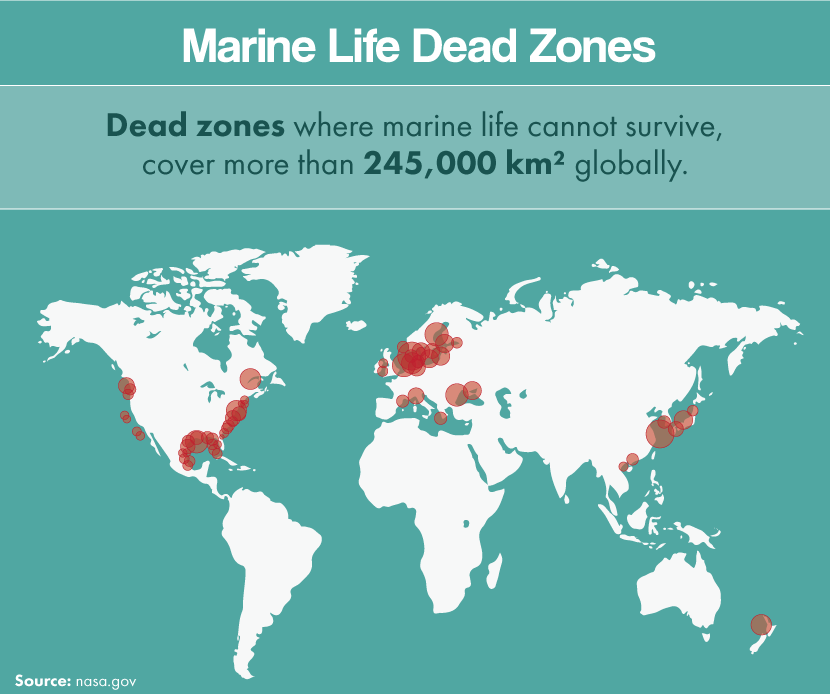
\includegraphics[width=300pt]{marine-life-dead-zones.png}
				\end{center}
				\caption{Répartition des zones mortes (source : nasa.gov)}
			\end{figure}
		
			On constate que certains pays dépassent en consommation la quantité d'eau renouvelable à disposition et exercent donc une pression sur le cycle de l'eau <sources>. \\
			La multitude de problématiques présentées ci-dessus explique pourquoi l'eau est au coeur des SDGs. Depuis de très nombreuses années, une attention particulière est portée à la qualité de l'eau et aux dangers liés à une contamination de celle-ci \cite{ashbolt_microbial_2004}. Le manque d'infrastructures sanitaires dans les régions en développement les rends vulnérables aux morts par contamination de l'eau. Neuf morts sur dix touchent les enfants. Aujourd'hui, de nombreux outils permettent de suivre avec précision les indicateurs classiques de qualité de l'eau tels que le taux d'oxygène, l'acidité, la température, la conductivité etc.
			Indicateurs SDG
			Satellites
			Le cas Suisse
		
		\subsubsection{Air}
			La qualité de l'air est aujourd'hui responsable de nombreuses maladies, cancers et décès. On estime
		\subsubsection{Territoire et cartographie}
		\subsubsection{Biodiversité}
	
	\subsection{Monitoring sociétal}
		\subsubsection{Santé}
		\subsubsection{Sécurité}
		\subsubsection{Développement}
		
\section{Participation citoyenne}
	\subsection{Standards}
	\subsection{Formation}
	\subsection{Récupération de données}
	\subsection{Traitement des données}
	\subsection{Outils}
		\subsubsection{Hardware}
		\subsubsection{Software}
		INatrualist, NatureBytes, Epicollect, SeeClickFix, Water Reporter, Project Noah		

\section{Projets}
	\subsection{Aqueduct}
	\subsection{InfoAmazonia}
	\subsection{World Water Monitoring Day}
	\subsection{Riverfly Monitoring Initiative}
	\subsection{Restoration Assessment Initiative}
	\subsection{Homebrew Sensing Project}
	\subsection{Open Water Project}
	\subsection{Open Air}
	\subsection{Open Land}
	\subsection{etc...}

\section{Conclusion}\label{sec:conclusion}

% use section* for acknowledgement
\section*{Remerciements}


\bibliographystyle{alpha}
\bibliography{soa} %%% soa.bib is the file containing bibliographic entries


% that's all folks
\end{document}


